\documentclass[aspectratio=169, xcolor=dvipsnames]{beamer}
\hypersetup{pdfpagemode=FullScreen}
\beamertemplatenavigationsymbolsempty
\setbeamertemplate{caption}{\raggedright\insertcaption\par}
\usepackage[utf8]{inputenc}
\usepackage[spanish]{babel}
\usepackage{siunitx}
\usepackage{graphicx}
\usepackage{xcolor}
\usepackage{amsmath}
\usepackage{esint}
\usepackage{biblatex}
\usepackage{multicol}
\usepackage{listings}

\definecolor{myblue}{rgb}{0.29, 0.5, 0.94}

\title{Aplicaciones de Sistemas Embebidos con Doble Núcleo}
\subtitle{Fundamentos de Programación para Sistemas Embebidos}
\author[Fabrizio Carlassara - Laboratorio de Sistemas Embebidos]{
\includegraphics[scale=0.15]{resources/images/utn_logo.png}}
\institute{UTN FRA\\Departamento de Ingeniería Electrónica\\Laboratorio de Sistemas Embebidos}
\date[]{\today} 
\usetheme{Warsaw}
\usecolortheme[named=myblue]{structure}
\setbeamertemplate{headline}{}

\begin{document}

\frame{\titlepage}
\begin{frame}{Fundamentos de Programación para Sistemas Embebidos}{Índice}
\begin{multicols}{2}
\tableofcontents
\end{multicols}
\end{frame}

\section{Periféricos}
\subsection{Generalidades}
\begin{frame}{Fundamentos de Programación para Sistemas Embebidos}{Generalidades}
\begin{columns}
    \begin{column}{0.5\textwidth}
    \begin{figure}
    \centering
    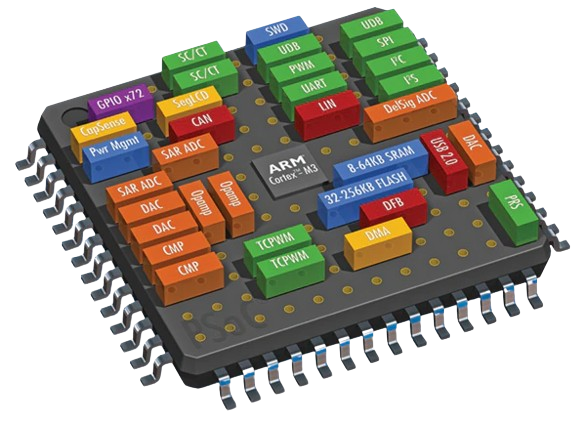
\includegraphics[width=1\linewidth]{resources/images/peripherals.png}
    \end{figure}
    \end{column}
    \begin{column}{0.5\textwidth}
    Periféricos comunes
    \noindent\rule{\textwidth}{0.5pt}
    \begin{itemize}
        \item General Purpose Input Output (GPIO)
        \item Analog to Digital Converter (ADC)
        \item Digital to Analog Converter (DAC)
        \item System Timer (Systick) y otros Timers
        \item Universal Synchronous Asynchronous Receiver Transmitter (USART)
        \item Inter-Integrated Circuit (I2C)
        \item Serial Peripherial Interface (SPI)
        \item Universal Serial Bus (USB)
    \end{itemize}
    \end{column}
\end{columns}
\end{frame}

\subsection{Configuración de pin}
\begin{frame}{Fundamentos de Programación para Sistemas Embebidos}{Configuración de pin}
\begin{columns}
\begin{column}{0.3\textwidth}
Cada pin tiene múltiples funciones asociadas. Se selecciona solo una de ellas de acuerdo a lo que se defina en la SWM y el IOCON.
\end{column}
\begin{column}{0.7\textwidth}
\begin{figure}
\centering
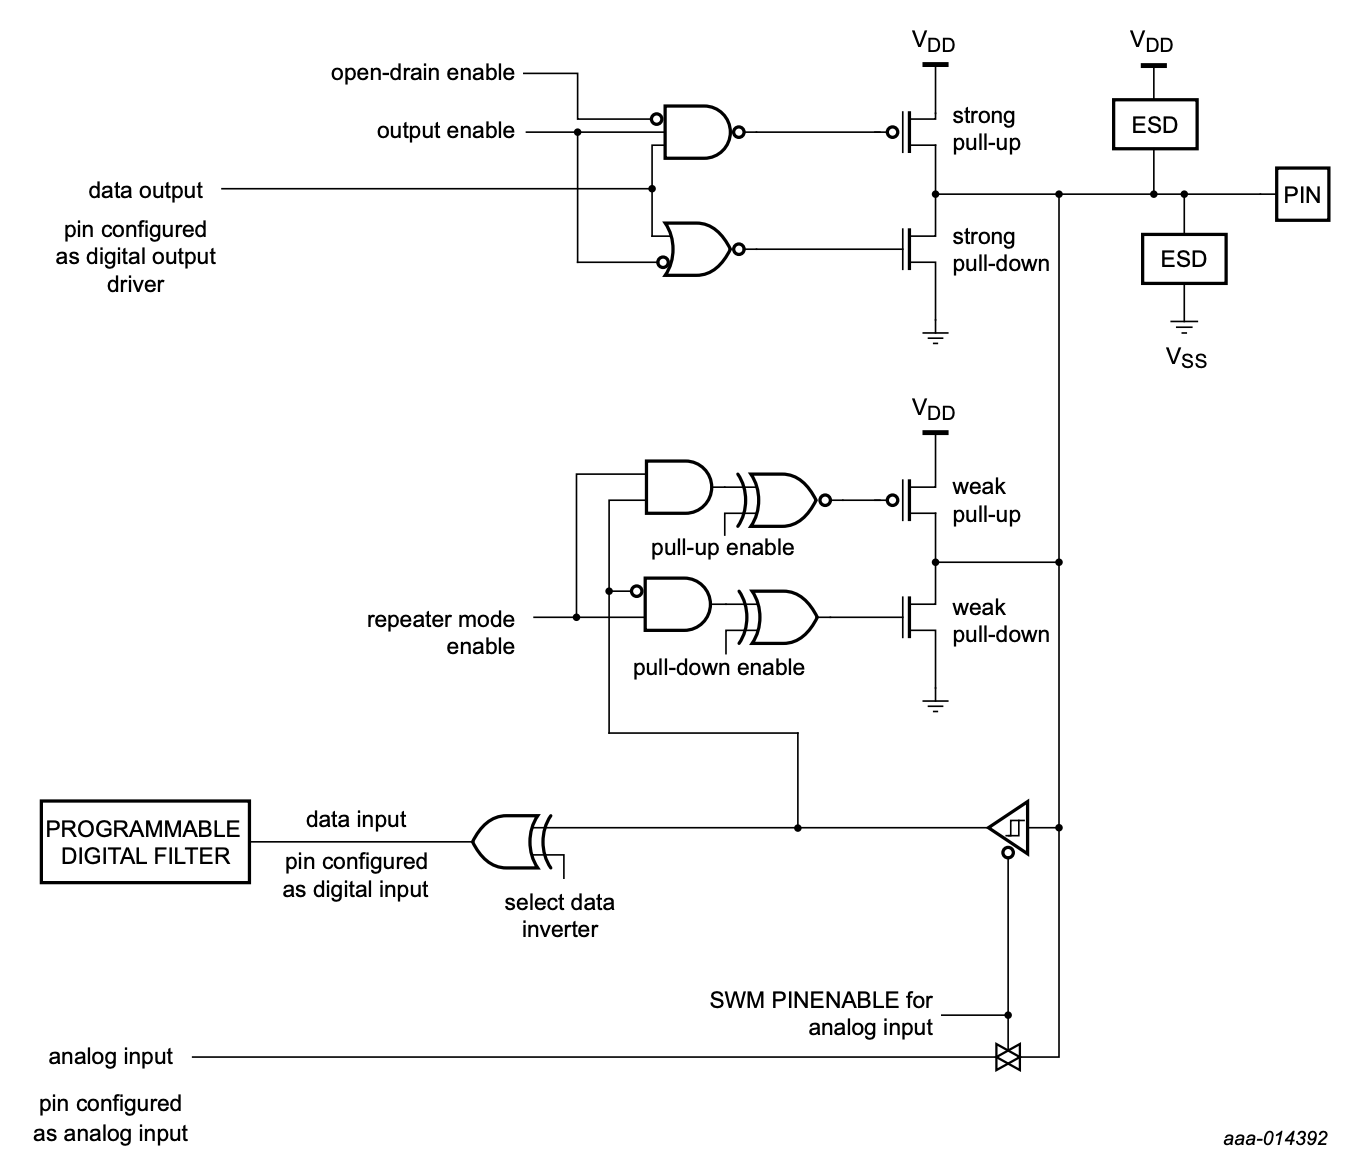
\includegraphics[width=0.75\linewidth]{resources/images/gpio_configuration.png}
\end{figure}    
\end{column}
\end{columns}
\end{frame}

\section{GPIO}
\subsection{Configuración de entrada}
\begin{frame}{Fundamentos de Programación para Sistemas Embebidos}{GPIO como entrada}
Uso típico
\noindent\rule{\textwidth}{0.5pt}
\begin{columns}
\begin{column}{0.55\textwidth}
\lstinputlisting[language=c, basicstyle=\tiny]{resources/listings/gpio_in.c}
\end{column}
\begin{column}{0.45\textwidth}
\begin{itemize}
    \item Se usa la estructura del tipo \textcolor{myblue}{gpio\_pin\_config\_t} con el valor \textcolor{myblue}{kGPIO\_DigitalInput}.
    \item La función \textcolor{myblue}{GPIO\_PortInit} permite habilitar el numero de puerto indicado.
    \item La función \textcolor{myblue}{GPIO\_PinInit} configura un pin en particular.
    \item Se usa \textcolor{myblue}{GPIO\_PinRead} para ver el estado del pin que será high (1) o low (0).
\end{itemize}
\end{column}
\end{columns}
\end{frame}

\subsection{Configuración de salida}
\begin{frame}{Fundamentos de Programación para Sistemas Embebidos}{GPIO como salida}
Uso típico
\noindent\rule{\textwidth}{0.5pt}
\begin{columns}
\begin{column}{0.4\textwidth}
\begin{itemize}
    \item Se usa la estructura del tipo \textcolor{myblue}{gpio\_pin\_config\_t} con el valor \textcolor{myblue}{kGPIO\_DigitalOutput}.
    \item Se puede en la estructura anterior, dar un valor de salida por defecto.
    \item Se usa \textcolor{myblue}{GPIO\_PinWrite} para escribir un valor en el pin que será high (1) o low (0).
\end{itemize}
\end{column}
\begin{column}{0.6\textwidth}
\lstinputlisting[language=c, basicstyle=\tiny]{resources/listings/gpio_out.c}
\end{column}
\end{columns}
\end{frame}

\section{ADC}
\subsection{Generalidades}
\begin{frame}{Fundamentos de Programación para Sistemas Embebidos}{Generalidades del ADC}
\begin{itemize}
    \item Convierten señales analógicas a valores discretos.
    \item Una resolución de 12 bits implica $2^{12}$ o 4096 valores discretos de resultado para una señal de 0 a 3,3V.
    \item Un total de 12 canales multiplexados.
    \item Velocidad de muestreo de 1,2Ms/s.
\end{itemize}
\begin{figure}
\centering
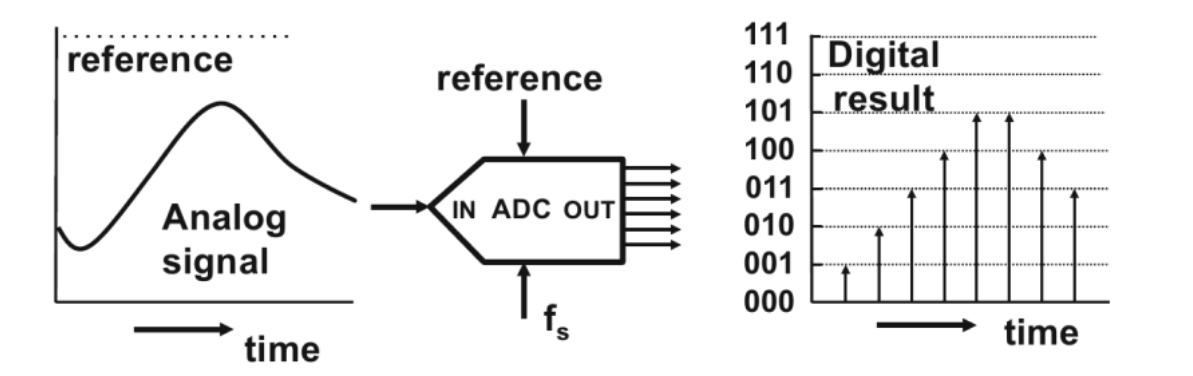
\includegraphics[width=0.75\linewidth]{resources/images/adc.png}
\end{figure}
\end{frame}

\subsection{Uso del ADC}
\begin{frame}{Fundamentos de Programación para Sistemas Embebidos}{Inicialización del ADC}
\begin{columns}
\begin{column}{0.5\textwidth}
\begin{itemize}
    \item Se elige la entrada analógica para el pin con \textcolor{myblue}{SWM\_SetFixedPinSelect}.
    \item Se elige la fuente de clock y prescaler del ADC con \textcolor{myblue}{CLOCK\_Select} y \textcolor{myblue}{CLOCK\_SetClkDivider}.
    \item Se alimenta el hardware del ADC con \textcolor{myblue}{POWER\_DisablePD}.
    \item Una calibración de clock es necesaria antes de inicializar el ADC, esto se hace con \textcolor{myblue}{ADC\_DoSelfCalibration}.
\end{itemize}
\end{column}
\begin{column}{0.5\textwidth}
\lstinputlisting[language=c, basicstyle=\tiny]{resources/listings/adc_init.c}
\end{column}
\end{columns}
\end{frame}

\begin{frame}{Fundamentos de Programación para Sistemas Embebidos}{Inicialización de una secuencia}
\begin{columns}
\begin{column}{0.5\textwidth}
\lstinputlisting[language=c, basicstyle=\tiny]{resources/listings/adc_init_sequence.c}
\end{column}
\begin{column}{0.5\textwidth}
\begin{itemize}
    \item Para por defecto el ADC usamos \textcolor{myblue}{ADC\_GetDefaultConfig} y \textcolor{myblue}{ADC\_Init}.
    \item Las secuencias son conversiones continuas de uno o muchos canales. Se configuran el/los canales en el campo \textcolor{myblue}{channelMask} de la estructura \textcolor{myblue}{adc\_conv\_seq\_config\_t}.
    \item Se pueden configurar fuentes de disparo y si las interrupciones son por canal o secuencia.
    \item La secuencia se configura y habilita con \textcolor{myblue}{ADC\_SetConvSeqAConfig} y \textcolor{myblue}{ADC\_EnableConvSeqA}.
\end{itemize}
\end{column}
\end{columns}
\end{frame}

\subsection{Lectura de secuencia}
\begin{frame}{Fundamentos de Programación para Sistemas Embebidos}{Lectura de una secuencia}
\begin{columns}
\begin{column}{0.5\textwidth}
\begin{itemize}
    \item Se inicia una secuencia de conversiones con \textcolor{myblue}{ADC\_DoSoftwareTriggerConvSeqA}.
    \item La función que devuelve el resultado de la conversión cuando está listo es \textcolor{myblue}{ADC\_GetChannelConversionResult} y requiere una estructura del tipo \textcolor{myblue}{adc\_result\_info\_t}.
    \item El valor del resultado se encuentra en el campo \textcolor{myblue}{result} de la estructura.
\end{itemize}
\end{column}
\begin{column}{0.5\textwidth}
\lstinputlisting[language=c, basicstyle=\tiny]{resources/listings/adc_read.c}
\end{column}
\end{columns}
\end{frame}

\section{DAC}
\subsection{Generalidades}
\begin{frame}{Fundamentos de Programación para Sistemas Embebidos}{Generalidades del DAC}
\begin{itemize}
    \item Convierten valores digitales en un registro a valores de tensión analógicos.
    \item Una resolución de 10 bits implica $2^{10}$ o 1024 valores analógicos posibles entre 0 y 3,3V.
    \item Dos salidas posibles con una tasa de refresco de hasta 1 MHz.
\end{itemize}
\begin{figure}
\centering
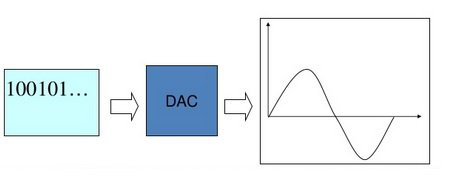
\includegraphics[width=0.5\linewidth]{resources/images/dac.png}
\end{figure}
\end{frame}

\subsection{Uso del DAC}
\begin{frame}{Fundamentos de Programación para Sistemas Embebidos}{Uso del DAC}
\begin{columns}
\begin{column}{0.5\textwidth}
\lstinputlisting[language=c, basicstyle=\tiny]{resources/listings/dac.c}
\end{column}
\begin{column}{0.5\textwidth}
\begin{itemize}
    \item Se usan funciones como \textcolor{myblue}{SWM\_SetFixedPinSelect} y \textcolor{myblue}{IOCON\_PinMuxSet} para elegir la función de DAC para un pin.
    \item El hardware DAC tiene que alimentarse con \textcolor{myblue}{POWER\_DisablePD}.
    \item Se configura el funcionamiento del DAC con \textcolor{myblue}{DAC\_Init} a partir de alguna estructura de configuración.
    \item Se usa \textcolor{myblue}{DAC\_SetBufferValue} para indicar un valor de 10 bits que se desea a la salida del DAC.
\end{itemize}
\end{column}
\end{columns}
\end{frame}

\section{Systick Timer}
\subsection{Generalidades}
\begin{frame}{Fundamentos de Programación para Sistemas Embebidos}{Generalidades del Systick Timer}
\begin{enumerate}
    \item Estándar en todos los Cortex-M y generan interrupciones cuando llega a cero el contador.
    \item Se pueden cargar valores de hasta $2^{24}$ en el contador y el valor cargado responde a $ticks = T_{systick} \times f_{systick}$.
\end{enumerate}
\begin{figure}
\centering
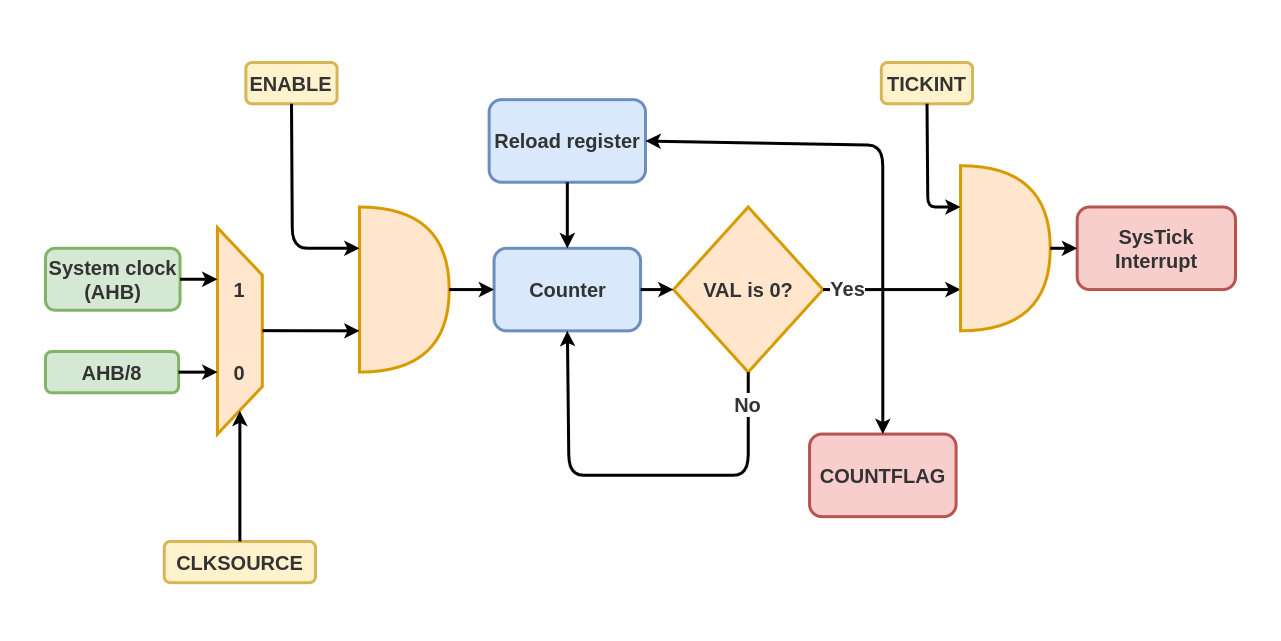
\includegraphics[width=0.6\linewidth]{resources/images/systick.png}
\end{figure}
\end{frame}

\subsection{Uso del Systick Timer}
\begin{frame}{Fundamentos de Programación para Sistemas Embebidos}{Configuración del Systick Timer}
\begin{columns}
\begin{column}{0.4\textwidth}
\lstinputlisting[language=c, basicstyle=\tiny]{resources/listings/systick.c}
\end{column}
\begin{column}{0.6\textwidth}
\begin{itemize}
    \item Se puede usar la variable \textcolor{myblue}{SystemCoreClock} para independizarse del valor de clock ya que esta variable tiene el valor del clock del CPU.
    \item Se puede dividir por la frecuencia deseada del Systick ($1ms = 1 / 1000$) para evitar el uso de números con decimales.
    \item Cada vez que se vence el Systick se llama al handler de una interrupción llamada \textcolor{myblue}{SysTick\_Handler}. Esta función se define por fuera del main.
\end{itemize}
\end{column}
\end{columns}
\end{frame}

\section{Ejercicios}
\begin{frame}{Fundamentos de Programación para Sistemas Embebidos}{Ejercicios}
    Algunas propuestas para practicar
    \noindent\rule{\textwidth}{0.75pt}
    \begin{enumerate}
        \item En un proyecto llamado \textbf{02\_systick\_blinky}, hacer un programa en el que el LED Azul parpadee cada 500ms y el LED D1 cada 1500ms.
        \item En un proyecto llamado \textbf{02\_custom\_blinky}, hacer un programa que haga que el LED Rojo parpadee de 100ms a 2s de acuerdo a lo indicado por el potenciómetro R22.
        \item En un proyecto llamado \textbf{02\_sine\_wave\_generator}, generar una senoidal de 1KHz de la mayor amplitud posible, con un offset de 1,65V en la salida PIO0\_29.
    \end{enumerate}
    \noindent\rule{\textwidth}{0.75pt}
    Cada ejercicio que se resuelva, subirlo al repositorio personal del curso.
\end{frame}

\section{Referencias}
\begin{frame}{Fundamentos de Programación para Sistemas Embebidos}{Referencias}
    Algunos recursos útiles
    \noindent\rule{\textwidth}{0.75pt}
    \begin{multicols}{2}
    \begin{itemize}
        \item \href{https://github.com/utn-fra-lse/lpc845/blob/main/docs/UM11029.pdf}{Manual del LPC845}
        \item \href{https://github.com/utn-fra-lse/lpc845/blob/main/docs/UM11181.pdf}{Manual del LPC845 Breakout Board}
        \item \href{https://mcuxpresso.nxp.com/api_doc/dev/116/modules.html}{Documentación del SDK del LPC845}
        \item \href{https://github.com/utn-fra-lse/lpc845/blob/main/docs/BASE_KIT_V0.pdf}{Esquemático del kit del laboratorio}
        \item \href{https://www.electronics-tutorials.ws/combination/analogue-to-digital-converter.html}{Analog to Digital Converter (ADC) Basics}
        \item \href{https://www.keil.com/pack/doc/CMSIS_Dev/Core/html/group__SysTick__gr.html}{Systick Timer}
        \href{https://developer.arm.com/documentation/101407/0540/Debugging/Debug-Windows-and-Dialogs/Core-Peripherals/Armv7-M-cores/Armv7-M--System-Tick-Timer}{Armv7-M System Tick Timer}
    \end{itemize}
    \end{multicols}
\end{frame}

\end{document}
